\documentclass[../main.tex]{subfiles}
%\usepackage{algorithm}
%\usepackage{algorithmic}
%\everymath{\displaystyle}
%\DeclareMathSizes{8}{8}{8}{8}
\def\arraystretch{2.0}
\begin{document}
\setlength{\delimitershortfall}{0pt}

\section{Derivatives of the fluid residual}\label{sec:dresidual_derivative}
This section is denoted to a thorough derivation of the partial derivatives $\pdfrac{\dresidual}{\dfstate}$ and $\pdfrac{\dresidual}{\absvar}$ of the fluid residual equation.
These are the main quantities needed in order to compute the sensitivity of the state vector $\tfrac{\dfstate}{\absvar}$ as shown in equation~\eqref{eq:full_sa_nostruct}.
We need this derivative in order to solve for $\tfrac{\optcrit_{j}}{\absvar_{i}}$.\\


\subsection{Fluid Jacobian $\pdfrac{\dresidual}{\dfstate}$}\label{sec:fluid_jacobian}





As described in~\eqref{eq:nse_final_discretized_notationchange}, the total residual is comprised of a convective(inviscid) part and a viscous contributions. Thanks to the distributive property of the derivative operator, we can thus compute the derivative of the total residual as the sum of the derivatives of the components. This is particulary important for us, since we used two different discretization routines for the viscous and the inviscid part.\\



\subsubsection{Derivative of the convective Jacobian $\pdfrac{\dresidual^c}{\dfstate}$}

Also, we will only discuss the special case of intersected elements in the following, since the special case of an non-intersected cell follows trivially from that.\\
For more details on the evaluation of the inviscid residual the reader is referred to section~\ref{sec:finite_volume_method}, specifically section~\ref{sec:mixed_FV_FE_formulation} and section~\ref{sec:fiver} for the incorporation of the immersed boundary conditions.


For the convective part of the Jacobian, $\dresidual^c$ we can be therefor write
\begin{align}
\dresidual^{c,i}_{ij} = \fluxesnum^i_{ij}(\dfstateprim_{ij},\dfstateprim^{*}_{ij},\normal_{ij})
\end{align}

Since the fluid normal is dependent on the mesh position this can also be written as
\begin{align}
\dresidual^{c,i}_{ij} = \fluxesnum^i_{ij}(\dfstateprim_{ij},\dfstateprim^{*}_{ij},\mpos)
\end{align}


If the edge $i-j$ is intersected however, the half-Riemann problem approach as discussed in section~\ref{sec:half_riemann_problem} is applied.
Also, the quantity $\dfstate_{ij}$ on the interface can be reconstructed in several ways. In this thesis we applied a \ac{MUSCL} technique. Of course, the reconstruction and limitation has to be taken into account as well.\\
Putting all this together, one can write

\begin{align}
    \frac{\partial \dresidual^{c,i}_{ij}}{\partial \dfstate_k} = 
    {\color{red}{\frac{\partial \dresidual^{c,i}_{ij}}{\partial \dfstateprim_{ij}^\star}}} \,
    {\color{blue}{\frac{\partial \dfstateprim_{ij}^\star}{\partial \dfstateprim_k}}} \,
    \frac{\partial \dfstateprim_k}{\partial \dfstate_k} +
    {\color{red}{\frac{\partial \dresidual^{c,i}_{ij}}{\partial \dfstateprim_{ij}}}} \,
    {\color{green}{\frac{\partial \dfstateprim_{ij}}{\partial \dfstateprim_k}}} \,
    \frac{\partial \dfstateprim_k}{\partial \dfstate_k} +
    \underbrace{\pdfrac{\dresidual^{c,i}_{ij}}{\dmpos}\pdfrac{\dmpos}{\normal_{ij}}}_{=\vec{0}\text{ for embedded}}
\end{align}

\begin{center}
	\begin{itemize}
	  \item {\color{red} {Analytical Jacobian of the (Roe's) centering flux} }
	  \item {\color{blue} {Analytical derivative of the solution of the 1D half-Riemann problem}}
	  \item {\color{green} {Analytical derivative of the MUSCL reconstruction and limitation}}
	\end{itemize}
\end{center}

where, $\prim{(\sim)}$ denotes primitive quantitives, $\frac{\partial \dfstateprim_k}{\partial \dfstate_k}$ accounts for the conversion between primitive and conservative state vector, $\pdfrac{\dresidual^{c,i}_{ij}}{\fstateprim^{\star}_{ij}}$ is the analytical derivative of the \ac{MUSCL} reconstruction and limitation and $a$ is the analytical Jacobian of the Roe flux. Finally, $\frac{\partial \dfstateprim_{ij}^\star}{\partial \dfstateprim_k}$ accounts for the analytical derivative of the solution of the 1D half-Riemann problem. This also accounts for the only really new derivative to be considered in comparison to the cells far from the immersed boundaries.\\
The analytic Jacobian of the Roe flux is provided in section~\ref{sec:jacobian_roeflux}, the derivative of the solution of the 1D half-Riemann problem is discussed in section~\ref{sec:fiver-1}, the derivative of the MUSCL reconstruction in section~\textbf{TODO} and finally, the derivative of the conversion to primitive variables is discussed in section~\textbf{TODO}.




\subsubsection{Derivative of the viscous Jacobian $\pdfrac{\dresidual^c}{\dfstate}$}\label{sec:jacobian_viscous}
For the discussion of the viscous Jacobian, we first remind the reader that an \ac{FE} approach is used to evaluate this term, in contrast to the \ac{FV} approach used for the inviscid contribution. For a detailed discussion the reader is referred to section~\ref{sec:mixed_FV_FE_formulation} and the following sections.\\
As far as the residual evaluation itself goes, we recall that, once the ghost points have been populated(see section~\ref{sec:ghost_node_reconstruction}}), the viscous residual is evaluated as though the cell had never been intersected in the first place.
We can therefore write the viscous residual of an intersected cell as


\begin{align}
    \dresidual^c(\dfstateprim^a,\dfstateprim^g(\dfstateprim^a))=\vec{0}
\end{align}
where $\dfstateprim^a$ represents the fluid states of the active node, and $\dfstateprim^g$ are the fluid states of the ghost nodes, which can themselves be expressed in terms of the active nodes.


Thus the derivative becomes:
\begin{align}
    \pdfrac{\dresidual^v(\dfstateprim^a,\dfstateprim^g(\dfstateprim^a))}{\dfstateprim}=
    \underbrace{\pdfrac{\dresidual^v}{\dfstateprim^a}}_{\substack{\text{can be re-used from ALE } \\ \text{after the ghost-point population}}}+
    \pdfrac{\dresidual^v}{\dfstateprim^g}\cdot
    \overbrace{\pdfrac{\dfstateprim^g}{\dfstateprim^a}}^{\substack{\text{obtained during the}\\ \text{population process} }}
\end{align}


For the analytic viscous Jacobian contribution we don't have to make a difference between $\pdfrac{\dresidual^c}{\dfstateprim^a}$ and $\pdfrac{\dresidual^v}{\dfstateprim^g}$.\\
We recall the definition of the viscous residual as
\begin{align}\label{eq:derivative_viscous_residual}
\dresidual_i^v=-\sum_{T_i \in \elementset(i)} \int_{T_j} \difftensor \nabla \dfstate \nabla \phi_j dx
\end{align}
again, we switch to primitive variables for easier evaluation

\begin{align}\label{eq:derivative_viscous_residual_primitives}
\dresidual_i^v=-\sum_{T_i \in \elementset(i)} \int_{T_j} \prim{\difftensor} \nabla \prim{\dfstate} \nabla \phi_j dx
\end{align}

Applying a numerical integration such as gauss rule, this becomes
\begin{align}\label{eq:aaa1}
\dresidual_i^v=-\sum_{T_i \in \elementset(i)} \sum_{i=1}^{n_g} 
w_i \prim{\difftensor} \nabla \prim{\dfstate}(\dmpos_i) \nabla \phi_j(\dmpos_i) dx
\end{align}

Thus, due the constant nature of the diffusive tensor $\difftensor$ the derivative can be written straightforwardly as
\begin{align}\label{eq:aaa2}
\pdfrac{\dresidual_i^v}{\prim{\dfstate}}=
-\sum_{T_i \in \elementset(i)} \sum_{i=1}^{n_g} 
w_i \prim{\difftensor} \nabla \prim{\dfstate}(\dmpos_i) \nabla \phi_j(\dmpos_i) dx
\end{align}




















\subsection{Analytic Jacobian of the Roe flux}\label{sec:jacobian_roeflux}

This section provides a detailed step by step derivation of the analytic convective Jacobian. This section is lengthy and not necessarily required for understanding the rest of the thesis. For this reason it has been moved at the end of this chapter. Nonetheless, in the authors opinion, it provides some crucial insight into the basics of \ac{SA}, and it is certainly of great help and serves as a reference for anyone who wants to implement those derivatives himself.\\

We start by expanding the derivative to
\begin{align}
\pdfrac{\dresidual_i^c}{\dfstate}=
\sum_{j \in \vertexset(i)}
\underbrace{\pdfrac{meas(C_{ij})}{\dfstate} \fluxesnum_{ij}(\dfstate_{ij},\dfstate_{ji},\wnormal_{ij})}_{=\vec{0}\text{ for embedded}} +
meas(C_{ij}) \pdfrac{\fluxesnum_{ij}(\dfstate_{ij},\dfstate_{ji},\wnormal_{ij})}{\dfstate}
\end{align}
where the first term is always zero for embedded simulations.\\
\question{TODO ask Farhat what to do with the first derivative.}

Next, we recall the definition of the numerical flux as
\begin{align}\label{eq:roe_flux}
\fluxesnum(\dfstate_i,\dfstate_j,\normal_{ij}) =
\frac{1}{2}\left[\fluxesconv(\dfstate_i)\cdot\normal_{ij} +
                 \fluxesconv(\dfstate_i)\cdot\normal_{ij}   \right] -
\frac{1}{2}\abs{\roeavgmat(\dfstate_i,\dfstate_j,\normal_{ij})} (\dfstate_j-\dfstate_i)
\end{align}

Similar to the \ac{MUSCL} procedure we transform the fluid state vector to primitive form
\begin{align}
\fstate=\begin{pmatrix}
        \dens \\ \dens\fluidvel \\ \energytot
        \end{pmatrix}
\overset{\mathsf{U}}{\mapsto}
\prim{\fstate}=\begin{pmatrix}
               \dens \\ \fluidvel \\ \pres
               \end{pmatrix}
\end{align}
Of course, this transformation involves the \ac{EOS} of the fluid. We will use $\prim{(\cdot)}$ from now on top mark any quantity as based on/formulated in primitive variables.\\
The primitive state vector is also much more appealing when it comes to the implementation of boundary conditions, since the solution variables are separated there.
 \\
Next we recall the conservative form of the Euler equations, which was presented in section~\ref{sec:conservative_form_nsg} as
\begin{align}\label{eq:t1}
\pdfrac{\fstate}{t}+\nabla\cdot\fluxesconv(\fstate)=\vec{0}
\end{align}
Where the convective flux matrix $\fluxesconv$ is provided in equation \eqref{eq:fluxesconv}, and can be written as
\begin{align}
\fluxesconv(\fstate)=\begin{pmatrix}
                      \fluxesconv_x(\fstate)&\fluxesconv_x(\fstate)&\fluxesconv_x(\fstate)
                      \end{pmatrix}
\end{align}
Therefore, applying the Nabla operator in equation \eqref{eq:t1} gives
\begin{align}\label{eq:euler_coinservative_splitted}
\pdfrac{\fstate}{t}+
\underbrace{\pdfrac{\fluxesconv_x(\fstate)}{\fstate}}_{\tensor{A}} \pdfrac{\fstate}{x} +
\underbrace{\pdfrac{\fluxesconv_y(\fstate)}{\fstate}}_{\tensor{B}} \pdfrac{\fstate}{y} +
\underbrace{\pdfrac{\fluxesconv_z(\fstate)}{\fstate}}_{\tensor{C}} \pdfrac{\fstate}{z}
=\vec{0}
\end{align}
where the matrices $\tensor{A}$,$\tensor{B}$ and $\tensor{C}$ are called the \expression{flux Jacobians}.
\end{document}

In Section~\ref{sec:SA}, we have derived that for any sensitivity calculation, the derivative of the flux matrix with respect to the fluid state vector $\pdfrac{\dresidual^c}{\fstate}$ is required.\\
We have derived in Section~\ref{sec:mixed_FV_FE_formulation} that at an interior vertex point of the fluid mesh, we have
\begin{align}\label{eq:convectiveterm _approximation2}
\left[\fluxmatconv(\dfstate,\dmpos,\dmms)\right]_i=
\sum_{j \in \vertexset(i)} mes(\partial C_{ij})\fluxesnum(\dfstate_i,\dfstate_j,\normal_{ij})
\end{align}
Since an equilibrium point is considered, $\dmms=\vec{0}$ and is neglected in the following derivations.

In equation~\eqref{eq:convectiveterm_approximation} we have introduced $\fluxesnum$ as the numerical flux function. In this thesis, we consider the popular Roe flux, which is defined as given in equation~\eqref{eq:roe_flux}.

Let us remind, that $\mathsf{R}_i^c$ is the convective residual at vertex $i$, $\vertexset(i)$ is the set of vertices connected to vertex $i$ by an edge, $C_i$ is the control volume of the dual cell centered at vertex $i$ and $\partial C_{ij}$ is the segment of the boundary that intersects edge $(ij)$ and $\wnormal_{ij}$ is the outward-facing weighted normal to $\partial C_{ij}$.
See figure~\ref{fig:dualcell_unstructured} for a visualization of the setup.
 \\
From Equation \eqref{eq:convectiveterm _approximation2} it is obvious that when looking for the derivative $\pdfrac{\fluxmatconv}{\dfstate}$, the derivative of the numerical flux with respect to the fluid state vector $\pdfrac{\fluxesnum}{\dfstate}$ is required.

To make things easier we will in the following derive the primitive version of that quantity $\pdfrac{\prim{\fluxesnum}}{\prim{\dfstate}}$
 \\
 \\
As \cite{Lesoinne2001} demonstrates, primitive version of the numerical Roe flux can be expressed as
\begin{align}\label{eq:primitive_roe_flux}
\prim{\fluxesnum}(\prim{\dfstate}_i,\prim{\dfstate}_j,\normal_{ij}) =
\frac{1}{2} \left(\prim{\fluxesconv}(\prim{\dfstate}_i)\cdot\normal_{ij} +
                  \prim{\fluxesconv}(\prim{\dfstate}_i)\cdot\normal_{ij}
            \right) -
\frac{1}{2} \inv{\jaceigvecs}(\sim)\abs{\jaceigvals(\sim)}\jaceigvecs(\sim)(\prim{\dfstate}_j-\prim{\dfstate}_i)
\end{align}


where, for ease of notation we omit the function arguments by simply writing $(\sim)$ as follows
\begin{align}\label{eq:split_roeaveragingmatrix}
\inv{\jaceigvecs}(\sim) &= \inv{\jaceigvecs}\left(\roeavgfunc(\sim),\normal_{ij}\right) \nonumber\\
\roeavgfunc(\sim)       &= \roeavgfunc\left(\prim{\fstate}_i,\prim{\fstate}_j\right)    \nonumber\\
\jaceigvals(\sim)       &= \jaceigvals\left(\roeavgfunc(\sim),\normal_{ij}\right)        \nonumber\\
\jaceigvecs(\sim)       &= \jaceigvecs\left(\roeavgfunc(\sim),\normal_{ij}\right)        \nonumber\\
\end{align}


\def\enthalp{\mathsf{H}}
Here, $\roeavgfunc(\prim{\fstate}_i,\prim{\fstate}_j)$  is the averaging function associated with the roe flux. It can be written as
\begin{align}
\roeavgfunc(\prim{\fstate}_i,\prim{\fstate}_j)=
\frac{1}{\sqrt{\rho_i}+\sqrt{\rho_j}}
\left(
\sqrt{\dens_i}
\begin{bmatrix}
\dens_i\\ \fluidvel_i \\ \enthalp_i
\end{bmatrix}
+
\sqrt{\dens_j}
\begin{bmatrix}
\dens_j \\ \fluidvel_j \\ \enthalp_j
\end{bmatrix}
\right)
\end{align}

and  $\jaceigvecs$ is the matrix whose columns are the right eigenvectors of the Jacobian matrix $\fluxjac$ of $\fluxesconv$.
The Jacobi matrix in primitive form can be written as



% Jacobian matrix of the flux %%%%%%%%%%%%%%%%%%%%%%%%%%%%%%%%%%%%%%%%%%%%%%%%%%%%%%%%%%%%%%%%%%%%%
\def\vn{\fluidvel\cdot\normal}
\def\jfo{H~(\vn)-\dens\vn \frac{\gamma\pres}{\dens(\gamma)}}
\def\jft{\dens\vn v_1+\dens H n_1}
\def\jftt{\dens\vn v_2+\dens H n_2}
\def\jff{\dens\vn v_3+\dens H n_3}
\def\jfff{\dens\vn\frac{\gamma}{\dens(\gamma-1)}}
\begin{align}
\prim{\fluxjac}&=\pdfrac{(\prim{\fluxesconv}\cdot\normal)}{\prim{\fstate}} \\
&=
\begin{bmatrix}
\vn      &  \dens n_x                &  \dens n_y                &  \dens n_z                 &  0   \\
v_1(\vn) &  \dens(\vn)+\dens v_1 n_1 &  \dens v_1 n_2            &  \dens v_1 n_3             &  n_1 \\
v_2(\vn) &  \dens v_2 n_1            &  \dens(\vn)+\dens v_2 n_2 &  \dens v_2 n_3             &  n_2 \\
v_3(\vn) &  \dens v_3 n_1            &  \dens v_3 n_2            &  \dens(\vn)+\dens v_3 n_3  &  n_2 \\
A_{51}   &  A_{52}                   &  A_{53}                   &  A_{54}                    & A_{55}
\end{bmatrix} \notag\\
&\fluxjac_{51}=\jfo  \notag\\
&\fluxjac_{52}=\jft  \notag\\
&\fluxjac_{53}=\jftt \notag\\
&\fluxjac_{54}=\jff  \notag\\
&\fluxjac_{55}=\jfff \notag\\
\end{align}


For this Jacobian, one can now symbolically derive an eigenvalue decomposition, such that
\begin{align}
\fluxjac=\inv{\jaceigvecs}\jaceigvals\jaceigvecs
\end{align}




The total specific enthalpy for a perfect gas is given as
\begin{align}
\enthalp=\frac{\specheatratio\pres}{\dens(\specheatratio-1)}+\frac{1}{2}\T{\fluidvel}\fluidvel
\end{align}
where we note the following derivatives
\begin{align}
\pdfrac{\enthalp}{\dens}=-\frac{\specheatratio\pres}{\dens^2(\specheatratio-1)}~~~~~~
\pdfrac{\enthalp}{\fluidvelcomp_i}=\fluidvelcomp_i~~~~~~
\pdfrac{\enthalp}{\pres}=\frac{\specheatratio}{\dens(\specheatratio-1)}
\end{align}

Therefore, the derivative of the averaging function with respect to the primitive fluid state vector can be calculated as
\def\sqdi{{\sqrt{\dens_{i}}}}
\def\sqdj{{\sqrt{\dens_{j} }}}
\def\Mwoneone{3\dens_i-\frac{\sqdi\dens_i+\sqdj\dens_j}{\sqdi+\sqdj}}
\def\Mwonetwo  {\fluidvelx_i-\frac{\sqdi\fluidvelx_i+\sqdj\fluidvelx_j}{\sqdi+\sqdj}}
\def\Mwonethree{\fluidvely_i-\frac{\sqdi\fluidvely_i+\sqdj\fluidvely_j}{\sqdi+\sqdj}}
\def\Mwonefour {\fluidvelz_i-\frac{\sqdi\fluidvelz_i+\sqdj\fluidvelz_j}{\sqdi+\sqdj}}
\def\Mwonefive{\frac{\T{\fluidvel}\fluidvel}{2}-\frac{\specheatratio\pres}{\dens(\specheatratio-1)}-\frac{\sqdi\enthalp_i+\sqdj\enthalp_j}{\sqdi+\sqdj}  }


\begingroup\makeatletter\def\f@size{8}\check@mathfonts
\def\maketag@@@#1{\hbox{\m@th\large\normalfont#1}}%
\begin{align}
\pdfrac{\roeavgfunc(\sim)}{\dens_i}&=
\frac{1}{2\sqrt{\dens_i}(\sqrt{\dens_i}+\sqrt{\dens_j})}
\left(
  -\roeavgfunc(\sim)+
  \T{\begin{bmatrix}
    3\dens_i & 2\sqrt{\dens_i}\fluidvel_i & 2\enthalp_i-2\dens_i\frac{\specheatratio\pres}{\dens^2(\specheatratio-1)}
  \end{bmatrix}}
\right)                                                                                                                      \notag\\
\pdfrac{\roeavgfunc(\sim)}{\fluidvelcomp_i}&=
\frac{1}{(\sqrt{\dens_i}+\sqrt{\dens_j})}\sqrt{\dens_i}
\T{\begin{bmatrix}
  0 & \T{\vec{e}_i} & \fluidvelcomp_i
\end{bmatrix}}                                                                                                               \notag\\
\pdfrac{\roeavgfunc(\sim)}{\pres_i} &=
\frac{1}{(\sqrt{\dens_i}+\sqrt{\dens_j})}\sqrt{\dens_i}
\T{\begin{bmatrix}
  0 & \T{\vec{0}} & \frac{\specheatratio}{\dens(\specheatratio-1)}
\end{bmatrix}}                                                                                                               \notag\\
\pdfrac{\roeavgfunc(\sim)}{\prim{\fstate}_i}&=
\begin{bmatrix}
  \Mwoneone  &  0                    &  0                    &  0                    & 0                                         \\
  \Mwonetwo   &  2\dens_i             &  0                    &  0                    & 0                                        \\
  \Mwonethree &  0                    &  2\dens_i             &  0                    & 0                                        \\
  \Mwonefour  &  0                    &  0                    &  2\dens_i             & 0                                        \\
  \Mwonefive  &  2\dens_i\fluidvelx_i &  2\dens_i\fluidvelx_i &  2\dens_i\fluidvelx_i & \frac{2\specheatratio}{\specheatratio-1} \\
\end{bmatrix}                                                                                                                      
\end{align}\endgroup


The matrix $\jaceigvecs$ can be written as
\def\gmo{\specheatratio-1}
\def\tone{\normal-\frac{(\gmo)\T{\fluidvel}\fluidvel }{2 c^2}\normal+\normal\times\fluidvel}
\begingroup\makeatletter\def\f@size{8}\check@mathfonts
\def\maketag@@@#1{\hbox{\m@th\large\normalfont#1}}%
\begin{align}
\jaceigvecs=
\begin{bmatrix}
\left(\tone\right)\cdot\vec{e}_1 &  \normalx(\gmo)\frac{\fluidvelx}{c^2} &  \normalx(\gmo)\frac{\fluidvely}{c^2}+\normalz &  \normalx(\gmo)\frac{\fluidvelz}{c^2}-\normaly  &  -\normalx\frac{\gmo}{c^2} \\
\left(\tone\right)\cdot\vec{e}_2 &  \normaly(\gmo)\frac{\fluidvelx}{c^2}-\normalz &  \normaly(\gmo)\frac{\fluidvely}{c^2} &  \normaly(\gmo)\frac{\fluidvelz}{c^2}+\normalx  &  -\normaly\frac{\gmo}{c^2} \\
\left(\tone\right)\cdot\vec{e}_3 &  \normalz(\gmo)\frac{\fluidvelx}{c^2}+\normaly &  \normalz(\gmo)\frac{\fluidvely}{c^2}-\normalx &  \normalz(\gmo)\frac{\fluidvelz}{c^2}  &  -\normaly\frac{\gmo}{c^2} \\
(\gmo)\frac{\T{\fluidvel}\fluidvel}{c^2}-c\fluidvel\cdot\normal & -(\gmo)\fluidvelx+c\normalx & -(\gmo)\fluidvely+c\normaly & -(\gmo)\fluidvelz+c\normalz & \gmo \\
(\gmo)\frac{\T{\fluidvel}\fluidvel}{c^2}-c\fluidvel\cdot\normal & -(\gmo)\fluidvelx-c\normalx & -(\gmo)\fluidvely-c\normaly & -(\gmo)\fluidvelz-c\normalz & \gmo \\
\end{bmatrix}
\end{align}\endgroup




where $c$ is the speed of sound given by $c=\sqrt{\frac{\specheatratio\pres}{\dens}}$

The matrix $\jaceigvals$ derives to
\begin{align}\label{eq:jaceigvals_definition}
\jaceigvals=
diag(\left[\fluidvel\cdot\normal,\fluidvel\cdot\normal,\fluidvel\cdot\normal,\fluidvel\cdot\normal+c,\fluidvel\cdot\normal-c)\right])
\end{align}



\begin{align}\label{eq:pdfrac_jaceigvalsBYfstate}
\pdfrac{\inv{\jaceigvecs}}{\fstateprim}(\fstateprim,\normal)\cdot b =
\left[
\pdfrac{r_1}{\fstateprim}(\fstateprim,\normal)\cdot b~~~~\cdots~~~~\pdfrac{r_5}{\fstateprim}(\fstateprim,\normal)\cdot b
\right]
\end{align}

\begin{align}\label{eq:pdfrac_jaceigvecsBYfstate_comp1}
\pdfrac{r_1}{\fstateprim}(\fstateprim,\normal)=
\begin{bmatrix}
0    &  0                    &  0                           &  0                           &  0 \\
0    &  \normal_x            &  0                           &  0                           &  0 \\
0    &  0                    &  \normal_x                   &  0                           &  0 \\
0    &  0                    &  0                           &  \normal_x                   &  0 \\
0    &  \fluidvelx\normalx  &  \fluidvely\normalx+\normalz &  \fluidvelz\normalx-\normaly &  0
\end{bmatrix}
\end{align}


\begin{align}\label{eq:pdfrac_jaceigvecsBYfstate_comp2}
\pdfrac{r_2}{\fstateprim}(\fstateprim,\normal)=
\begin{bmatrix}
0    &  0                             &  0                  &  0                           &  0 \\
0    &  \normal_y                     &  0                  &  0                           &  0 \\
0    &  0                             &  \normal_y          &  0                           &  0 \\
0    &  0                             &  0                  &  \normal_y                   &  0 \\
0    &  \fluidvelx\normaly-\normalz   &  \fluidvely\normaly &  \fluidvelz\normaly-\normalx &  0
\end{bmatrix}
\end{align}


\begin{align}\label{eq:pdfrac_jaceigvecsBYfstate_comp3}
\pdfrac{r_3}{\fstateprim}(\fstateprim,\normal)=
\begin{bmatrix}
0    &  0                             &  0                           &  0                  &  0 \\
0    &  \normal_z                     &  0                           &  0                  &  0 \\
0    &  0                             &  \normal_z                   &  0                  &  0 \\
0    &  0                             &  0                           &  \normal_z          &  0 \\
0    &  \fluidvelx\normalz+\normaly   &  \fluidvely\normalz-\normalx &  \fluidvelz\normalz &  0
\end{bmatrix}
\end{align}



\begin{align}\label{eq:pdfrac_jaceigvecsBYfstate_comp4}
\pdfrac{r_4}{\fstateprim}(\fstateprim,\normal)=
\begin{bmatrix}
\frac{1}{2\specheatratio\pres}                            &  0                   &  0                   &  0              & -\frac{\dens}{2\gamma\pres^2}                             \\
\frac{\fluidvelx}{2\dens c^2} + \frac{\normalx}{4\dens c} &  \frac{1}{2 c^2}     &  0                   &  0              &  -\frac{\fluidvelx}{2\pres c^2}-\frac{\normalx}{4\pres c} \\
\frac{\fluidvely}{2\dens c^2} + \frac{\normaly}{4\dens c} &  0                   &  \frac{1}{2 c^2}     &  0              &  -\frac{\fluidvely}{2\pres c^2}-\frac{\normaly}{4\pres c} \\
\frac{\fluidvelz}{2\dens c^2} + \frac{\normalz}{4\dens c} &  0                   &  0                   & \frac{1}{2 c^2} &  -\frac{\fluidvelz}{2\pres c^2}-\frac{\normalz}{4\pres c} \\
\frac{1}{2\specheatratio}+\frac{\fluidvel\cdot\normal}{4\dens c} & \frac{\normalx}{2 c} & \frac{\normaly}{2 c} & \frac{\normalz}{2 c} & -\frac{\fluidvel\cdot\normal}{4\pres c}
\end{bmatrix}
\end{align}

\begin{align}\label{eq:pdfrac_jaceigvecsBYfstate_comp5}
\pdfrac{r_5}{\fstateprim}(\fstateprim,\normal)=
\begin{bmatrix}
\frac{1}{2\specheatratio\pres}                            &  0                   &  0                   &  0              & -\frac{\dens}{2\gamma\pres^2}                             \\
\frac{\fluidvelx}{2\dens c^2} - \frac{\normalx}{4\dens c} &  \frac{1}{2 c^2}     &  0                   &  0              &  -\frac{\fluidvelx}{2\pres c^2}+\frac{\normalx}{4\pres c} \\
\frac{\fluidvely}{2\dens c^2} - \frac{\normaly}{4\dens c} &  0                   &  \frac{1}{2 c^2}     &  0              &  -\frac{\fluidvely}{2\pres c^2}+\frac{\normaly}{4\pres c} \\
\frac{\fluidvelz}{2\dens c^2} - \frac{\normalz}{4\dens c} &  0                   &  0                   & \frac{1}{2 c^2} &  -\frac{\fluidvelz}{2\pres c^2}+\frac{\normalz}{4\pres c} \\
\frac{1}{2\specheatratio}-\frac{\fluidvel\cdot\normal}{4\dens c} & -\frac{\normalx}{2 c} & -\frac{\normaly}{2 c} & -\frac{\normalz}{2 c} & \frac{\fluidvel\cdot\normal}{4\pres c}
\end{bmatrix}
\end{align}

Due to its shape, the derivation of $\jaceigvals$ can be simplified to a differentiation of the eigenvalues $\eigval_i$.
\begin{align}\label{eq:pdfrac_jaceigvalsBYfstate}
\pdfrac{\eigval_1}{\fstateprim}(\fstateprim,\normal)&=\pdfrac{\eigval_2}{\fstateprim}(\fstateprim,\normal)=\pdfrac{\eigval_3}{\fstateprim}(\fstateprim,\normal)=
\T{\left[
0~~~~\T{\normal}~~~~0
\right] } \\
\pdfrac{\eigval_4}{\fstateprim}(\fstateprim,\normal)&=
\T{\left[
-\frac{c}{2\dens}~~~~\T{\normal}~~~~\frac{c}{2 \pres}
\right] } \\
\pdfrac{\eigval_5}{\fstateprim}(\fstateprim,\normal)&=
\T{\left[
\frac{c}{2\dens}~~~~\T{\normal}~~~~-\frac{c}{2 \pres}
\right] }
\end{align}



\begin{align}\label{eq:pdfrac_jaceigvalsBYfstate_comp1}
\pdfrac{\jaceigvecs}{\fstateprim}(\fstateprim,\normal)\cdot b=
\begin{bmatrix}
\pdfrac{\T{l_1}}{\fstateprim}(\fstateprim,\normal)\cdot b \\
\pdfrac{\T{l_2}}{\fstateprim}(\fstateprim,\normal)\cdot b \\
\pdfrac{\T{l_3}}{\fstateprim}(\fstateprim,\normal)\cdot b \\
\pdfrac{\T{l_4}}{\fstateprim}(\fstateprim,\normal)\cdot b \\
\pdfrac{\T{l_5}}{\fstateprim}(\fstateprim,\normal)\cdot b \\
\end{bmatrix}
\end{align}

\begin{align}\label{eq:pdfrac_jaceigvalsBYfstate_comp1}
\pdfrac{l_1}{\fstateprim}(\fstateprim,\normal)=
\begin{bmatrix}
-\frac{\normalx(\gmo)\norm{\fluidvel}^2}{2\dens\sspeed^2} & -\frac{\normalx(\gmo)\fluidvelx}{\sspeed^2}        & -\frac{\normalx(\gmo)\fluidvely}{\sspeed^2}-\normalz & -\frac{\normalx(\gmo)\fluidvelz}{\sspeed^2}+\normaly & \frac{\normalx(\gmo)\norm{\fluidvel}^2}{2\dens\sspeed^2} \\
\frac{\normalx(\gmo)\fluidvelx}{\specheatratio\pres} & \frac{\normalx\dens(\gmo)}{\specheatratio\pres} & 0 & 0 & -\frac{\normalx\fluidvelx\dens(\gmo)}{\specheatratio\pres^2} \\
\frac{\normalx(\gmo)\fluidvely}{\specheatratio\pres} & 0 & \frac{\normalx\dens(\gmo)}{\specheatratio\pres} & 0 & -\frac{\normalx\fluidvely\dens(\gmo)}{\specheatratio\pres^2} \\
\frac{\normalx(\gmo)\fluidvelz}{\specheatratio\pres} & 0 & 0 &\frac{\normalx\dens(\gmo)}{\specheatratio\pres}  & -\frac{\normalx\fluidvelz\dens(\gmo)}{\specheatratio\pres^2} \\
-\frac{\normalx\gmo}{\dens\sspeed^2}                 & 0 & 0 & 0                                               &  \frac{\normalx\gmo}{\pres\sspeed^2}
\end{bmatrix}
\end{align}

\begin{align}\label{eq:pdfrac_jaceigvalsBYfstate_comp2}
\pdfrac{l_2}{\fstateprim}(\fstateprim,\normal)=
\begin{bmatrix}
-\frac{\normaly(\gmo)\norm{\fluidvel}^2}{2\dens\sspeed^2} & -\frac{\normaly(\gmo)\fluidvelx}{\sspeed^2}+\normalz        & -\frac{\normaly(\gmo)\fluidvely}{\sspeed^2} & -\frac{\normaly(\gmo)\fluidvelz}{\sspeed^2}-\normalx & \frac{\normaly(\gmo)\norm{\fluidvel}^2}{2\dens\sspeed^2} \\
\frac{\normaly(\gmo)\fluidvelx}{\specheatratio\pres} & \frac{\normaly\dens(\gmo)}{\specheatratio\pres} & 0 & 0 & -\frac{\normaly\fluidvelx\dens(\gmo)}{\specheatratio\pres^2} \\
\frac{\normaly(\gmo)\fluidvely}{\specheatratio\pres} & 0 & \frac{\normaly\dens(\gmo)}{\specheatratio\pres} & 0 & -\frac{\normaly\fluidvely\dens(\gmo)}{\specheatratio\pres^2} \\
\frac{\normaly(\gmo)\fluidvelz}{\specheatratio\pres} & 0 & 0 &\frac{\normaly\dens(\gmo)}{\specheatratio\pres}  & -\frac{\normaly\fluidvelz\dens(\gmo)}{\specheatratio\pres^2} \\
-\frac{\normaly\gmo}{\dens\sspeed^2}                 & 0 & 0 & 0                                               &  \frac{\normaly\gmo}{\pres\sspeed^2}
\end{bmatrix}
\end{align}

\begin{align}\label{eq:pdfrac_jaceigvalsBYfstate_comp3}
\pdfrac{l_3}{\fstateprim}(\fstateprim,\normal)=
\begin{bmatrix}
-\frac{\normalz(\gmo)\norm{\fluidvel}^2}{2\dens\sspeed^2} & -\frac{\normalz(\gmo)\fluidvelx}{\sspeed^2}-\normaly        & -\frac{\normalz(\gmo)\fluidvely}{\sspeed^2}+\normalx & -\frac{\normalz(\gmo)\fluidvelz}{\sspeed^2} & \frac{\normalz(\gmo)\norm{\fluidvel}^2}{2\dens\sspeed^2} \\
\frac{\normalz(\gmo)\fluidvelx}{\specheatratio\pres} & \frac{\normalz\dens(\gmo)}{\specheatratio\pres} & 0 & 0 & -\frac{\normalz\fluidvelx\dens(\gmo)}{\specheatratio\pres^2} \\
\frac{\normalz(\gmo)\fluidvely}{\specheatratio\pres} & 0 & \frac{\normaly\dens(\gmo)}{\specheatratio\pres} & 0 & -\frac{\normalz\fluidvely\dens(\gmo)}{\specheatratio\pres^2} \\
\frac{\normalz(\gmo)\fluidvelz}{\specheatratio\pres} & 0 & 0 &\frac{\normaly\dens(\gmo)}{\specheatratio\pres}  & -\frac{\normalz\fluidvelz\dens(\gmo)}{\specheatratio\pres^2} \\
-\frac{\normalz\gmo}{\dens\sspeed^2}                 & 0 & 0 & 0                                               &  \frac{\normalz\gmo}{\pres\sspeed^2}
\end{bmatrix}
\end{align}

\begin{align}\label{eq:pdfrac_jaceigvalsBYfstate_comp4}
\pdfrac{l_4}{\fstateprim}(\fstateprim,\normal)=
\begin{bmatrix}
\frac{\sspeed}{2\dens}\fluidvel\cdot\normal & (\gmo)\fluidvelx-\sspeed\normalx & (\gmo)\fluidvely-\sspeed\normaly & (\gmo)\fluidvelz-\sspeed\normalz & -\frac{\sspeed}{2\pres}\fluidvel\cdot\normal \\
-\frac{\sspeed\normalx}{2\dens} &  -(\gmo) &  0       &  0       &  \frac{\sspeed\normalx}{2\pres} \\
-\frac{\sspeed\normaly}{2\dens} &  0       &  -(\gmo) &  0       &  \frac{\sspeed\normaly}{2\pres} \\
-\frac{\sspeed\normalz}{2\dens} &  0       &  0       &  -(\gmo) &  \frac{\sspeed\normalz}{2\pres} \\
0                               &  0       &  0       &  0       &  0                              \\
\end{bmatrix}
\end{align}


\begin{align}\label{eq:pdfrac_jaceigvalsBYfstate_comp5}
\pdfrac{l_5}{\fstateprim}(\fstateprim,\normal)=
\begin{bmatrix}
\frac{\sspeed}{2\dens}\fluidvel\cdot\normal & (\gmo)\fluidvelx-\sspeed\normalx & (\gmo)\fluidvely-\sspeed\normaly & (\gmo)\fluidvelz-\sspeed\normalz & -\frac{\sspeed}{2\pres}\fluidvel\cdot\normal \\
\frac{\sspeed\normalx}{2\dens} &  -(\gmo) &  0       &  0       &  -\frac{\sspeed\normalx}{2\pres} \\
\frac{\sspeed\normaly}{2\dens} &  0       &  -(\gmo) &  0       &  -\frac{\sspeed\normaly}{2\pres} \\
\frac{\sspeed\normalz}{2\dens} &  0       &  0       &  -(\gmo) &  -\frac{\sspeed\normalz}{2\pres} \\
0                              &  0       &  0       &  0       &  0                               \\
\end{bmatrix}
\end{align}

Therefor, the numerical roe flux~\eqref{eq:primitive_roe_flux} can therefore be derived by the primitive state vector as:

\def\jaceigvalssim{\abs{\jaceigvals(\sim)}}
\def\jaceigvecssim{\jaceigvecs(\sim)}
\def\invjaceigvecssim{\inv{\jaceigvecs}(\sim)}
\def\pdabsjaceigvalsBYw{\pdfrac{\abs{\jaceigvals}}{\fstateprim}(\sim)}
\def\pdroeavgBYw{\pdfrac{\roeavgfunc}{\fstateprim}(\sim)}
\def\wdiff{(\fstateprim_j-\fstateprim_i)}

\def\pdinvjaceigvecsBYw{\pdfrac{\inv{\jaceigvecs}}{\prim{\fstate}}(\sim)}
\def\pdjaceigvecsBYw{\pdfrac{\jaceigvecs}{\prim{\fstate}}(\sim)}
\begin{align}
\pdfrac{\prim{\fluxesnum}}{\prim{\fstate_i}}&=
\frac{1}{2}\fluxjac(\prim{\fstate}_i,\prim{\fstate}_j)\\
&-\frac{1}{2}\Bigg[
  \Big( \pdinvjaceigvecsBYw \pdroeavgBYw \Big)
  \jaceigvalssim \jaceigvecssim \wdiff
  \\ &~~+
  \invjaceigvecssim \Big( \pdabsjaceigvalsBYw \pdroeavgBYw \Big)
  \jaceigvecssim \wdiff  
  \\ &~~+
  \invjaceigvecssim \jaceigvalssim \Big( \pdjaceigvecsBYw\pdroeavgBYw \Big) \wdiff
  \\ &~~-
  \invjaceigvecssim \jaceigvalssim \jaceigvecssim
\Bigg]
\end{align}
where the full analytic expression can be obtained by backward substitution of equations~\eqref{eq:split_roeaveragingmatrix} to \eqref{eq:pdfrac_jaceigvalsBYfstate_comp5}.\\
This derivative, along with the derivative of the viscous term, which will be derived in Section~\ref{sec:derivative_viscous_residual}, will be a key component in the Sensitivity calculations as shown in Section~\ref{sec:SA} and \ref{sec:aeroelastic_sa}. This is due to the fact that will follow the procedere of discretization before derivation as justified in Section~\ref{sec:discretization_vs_differentiation}.







\subsection{Derivative with respect to the abstract variable $\pdfrac{\dresidual}{\absvar}$}\label{sec:dresidual_by_absvar}
Since the fluid Jacobian is also required in every standard fluid solve, the important term, unique to \ac{SA} is the partial derivative of the residual with respect to the design variable $\absvar$.\\
Similar to the previously discussed fluid Jacobian, the computation of $\pdfrac{\dresidual}{\absvar}$ can be splitted into convective and viscous part.
We again focus on the special case of an intersected cell in the following two subsections, since the standard case of a standard cell far from the interface follows trivially from that.

It shall also be noted that in most cases, the derivative $\pdfrac{\dresidual}{\absvar}$ is non-zero only at a few fluid nodes. For shape-sensitivity, for example, only the nodes at the interface have a non-zero contribution here. Looking at equation \eqref{eq:full_sa_nostruct} one can therefor interpret the solution of the linear system, or the multiplication with the inverse Jacobian, as a propagation operation.\\
\subsubsection{Convective contribution $\pdfrac{\dresidual^c}{\absvar}$}
Generally, one can write the convective fluid residual as 
\begin{align}\label{eq:convective_residual_fulldependency}
\dresidual^{c,i}_{ij} = \fluxesnum^i_{ij}(\dfstateprim_{ij},\dfstateprim^{*}_{ij}(\absvar),\normal_{ij})
\end{align}
The most important factor here, is of course the dependency of the half Riemann solution on the abstract variable. This dependecy becomes obvious in the case of shape sensitivity, since the intersection point used for the Riemann solution depends upon the interface shape.\\
The derivative can be obtained straightforwardly as
\begin{align}
\dresidual{\dresidual^{c,i}_{ij}}{\absvar}=\pdfrac{\dresidual^{c,i}_{ij}}{\dfstate^{\star}_{ij}}\pdfrac{\dfstate^{\star}_{ij}}{\absvar}
\end{align}
here, the analytical derivative of the first term can be taken from section \ref{sec:fluid_jacobian}.
The second derivative is more cumbersome. The issue is visualized in Figure~\ref{fig:pierce}.

\begin{figure}[!ht]
\centering
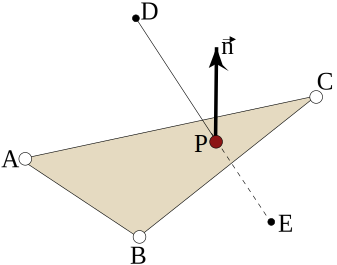
\includegraphics[width=0.3\linewidth]{\mainpath/fig/pdf/pierce}
\caption[Visualization of a face intersection in 3D]{Visualization of the intersection of a fluid mesh edge $(D-E)$ with an element of the embedded surface $(A-B-C)$. For a shape-sensitivity analysis, SDesign returns the derivatives of the embedded surface nodes $A,B,C$ position with respect to the shape parameter. This is done by first computing the intersection point $P$. Together with the element normal $\normal$, the intersection point is used to reconstruct the shape derivatives at nodes $D$ and $E$. \textbf{TODO}}
\label{fig:pierce}
\end{figure}

Based on the consideration above, we find the following dependency for the 
\begin{align}
\pdfrac{\dfstate^{\star}_{ij}}{\absvar}=\pdfrac{\dfstate^{\star}_{ij}}{\absvar}
\Big(
\pdfrac{\dfstate_{i}}{\absvar}\rvert_{i=A,B,C},\xi,\normal
\Big)
\end{align}

The derivatives of the geometrical quantities with respect to $\absvar$ are found as
\begin{align}
\pdfrac{\xi}{\absvars}&=\pdfrac{\xi}{\mpos}\pdfrac{\mpos}{\absvars} \\
\pdfrac{\normal_{wall}}{\absvar}&=\pdfrac{\normal_{wall}}{\mpos}\pdfrac{\mpos}{\absvar}
\end{align}


\subsubsection{Viscous contribution $\pdfrac{\dresidual^v}{\absvar}$}
The derivative of the viscous contibution is derived very simmilarly to the viscous Jacobian.
Looking at equation \textbf{TODO} one can derive
\begin{align}
    \pdfrac{\dresidual^v(\absvars,\dfstateprim^a(\absvars),\dfstateprim^g(\dfstateprim^a(\absvars)),\mpos(\absvars))}{\absvars}=
    &\underbrace{\pdfrac{\dresidual^v}{\dfstateprim^a}\pdfrac{\dfstateprim^a}{\absvars}}_{\substack{\text{can be re-used from ALE } \\ \text{after the ghost-point population}}}+
    \pdfrac{\dresidual^v}{\dfstateprim^g}\cdot
    \overbrace{\pdfrac{\dfstateprim^g}{\dfstateprim^a}}^{\substack{\text{obtained during the}\\ \text{population process} }} \pdfrac{\dfstateprim^a}{\absvars} \nonumber \\
    &+
    \underbrace{\pdfrac{\dresidual}{\dmpos}\pdfrac{\dmpos}{\absvars}}_{=\vec{0}\text{ for embedded}}
\end{align}



